
\documentclass{beamer}

\mode<presentation>
{
  \usetheme{Boadilla}      
  \usecolortheme{beaver}
  \usefonttheme{professionalfonts}  
  \setbeamertemplate{navigation symbols}{}
  \setbeamertemplate{caption}[numbered]
} 

\usepackage[english]{babel}
\usepackage[utf8x]{inputenc}
\usepackage{graphicx}
\usepackage{listings}
\usepackage{color}
\usepackage{tikz}
\usepackage{float}
\usepackage{ulem}
\usepackage{setspace}
\usepackage{perpage} %the perpage package
\usepackage{multicol}
\MakePerPage{footnote} %the perpage package command

\makeatletter
\newenvironment{btHighlight}[1][]
{\begingroup\tikzset{bt@Highlight@par/.style={#1}}\begin{lrbox}{\@tempboxa}}
{\end{lrbox}\bt@HL@box[bt@Highlight@par]{\@tempboxa}\endgroup}

\newcommand\btHL[1][]{%
  \begin{btHighlight}[#1]\bgroup\aftergroup\bt@HL@endenv%
}
\def\bt@HL@endenv{%
  \end{btHighlight}%   
  \egroup
}
\newcommand{\bt@HL@box}[2][]{%
  \tikz[#1]{%
    \pgfpathrectangle{\pgfpoint{1pt}{0pt}}{\pgfpoint{\wd #2}{\ht #2}}%
    \pgfusepath{use as bounding box}%
    \node[anchor=base west, fill=orange!30,outer sep=0pt,inner xsep=0pt, inner ysep=-1pt, rounded corners=3pt, minimum height=\ht\strutbox+1pt,#1]{\raisebox{1pt}{\strut}\strut\usebox{#2}};
  }%
}
\makeatother

\definecolor{mygreen}{rgb}{0,0.6,0}
\definecolor{mygray}{rgb}{0.5,0.5,0.5}
\definecolor{mymauve}{rgb}{0.58,0,0.82}
\definecolor{myblue}{rgb}{0,0,0.5}
\definecolor{keywordcolor}{RGB}{51, 102, 255}
\definecolor{myorange}{RGB}{230, 92, 0}

\lstset{ %
  backgroundcolor=\color{white},   % choose the background color; you must add \usepackage{color} or \usepackage{xcolor}; should come as last argument
  basicstyle=\ttfamily\tiny\color{myblue},        % the size of the fonts that are used for the code
  breakatwhitespace=false,         % sets if automatic breaks should only happen at whitespace
  breaklines=true,                 % sets automatic line breaking
  captionpos=b,                    % sets the caption-position to bottom
  commentstyle=\color{mygreen},    % comment style
  deletekeywords={...},            % if you want to delete keywords from the given language
  escapeinside={\%*}{*)},          % if you want to add LaTeX within your code
  extendedchars=true,              % lets you use non-ASCII characters; for 8-bits encodings only, does not work with UTF-8
  frame=none,                    % adds a frame around the code
  keepspaces=true,                 % keeps spaces in text, useful for keeping indentation of code (possibly needs columns=flexible)
  keywordstyle=\color{keywordcolor},       % keyword 
  language=Java,                 % the language of the code
  morekeywords={*,...},           % if you want to add more keywords to the set
  numbers=none,                    % where to put the line-numbers; possible values are (none, left, right)
  numbersep=10pt,                   % how far the line-numbers are from the code
  numberstyle=\tiny\color{mygray}, % the style that is used for the line-numbers  
  rulecolor=\color{mygray},         % if not set, the frame-color may be changed on line-breaks within not-black text (e.g. comments (green here))
  showspaces=false,                % show spaces everywhere adding particular underscores; it overrides 'showstringspaces'
  showstringspaces=false,          % underline spaces within strings only
  showtabs=false,                  % show tabs within strings adding particular underscores
  stepnumber=1,                    % the step between two line-numbers. If it's 1, each line will be numbered
  stringstyle=\color{myorange},     % string literal style
  tabsize=2,                     % sets default tabsize to 2 spaces
  title=\lstname,                   % show the filename of files included with \lstinputlisting; also try caption instead of title
  moredelim=**[is][\btHL]{`}{`},
  moredelim=**[is][{\btHL[fill=orange!30,draw=red]}]{@}{@},
}


\lstdefinestyle{Java}{
    language={Java},
    moredelim=**[is][\btHL]{`}{`},
    moredelim=**[is][{\btHL[fill=orange!30,draw=red]}]{@}{@},
}

\lstdefinelanguage{docker-compose-2}{  
  keywords={version, volumes, services},
  keywordstyle=\color{blue}\bfseries,
  keywords=[2]{image, environment, ports, container_name, ports, links, build},
  keywordstyle=[2]\color{olive}\bfseries,
  identifierstyle=\color{black},
  sensitive=false,
  comment=[l]{\#},
  commentstyle=\color{purple}\ttfamily,
  stringstyle=\color{red}\ttfamily,
  morestring=[b]',
  morestring=[b]"
}


\title[Docker]{Docker 101}
\author{Denis Timofeev}
\date{Feb 07, 2019}

\begin{document}

\AtBeginSection[]
{
  \begin{frame}<beamer>
    \frametitle{Outline}
    \begin{multicols}{2}
    \tableofcontents[
      currentsection
    ]
    \end{multicols}
  \end{frame}
}

\begin{frame}
  \titlepage
\end{frame}

\section{Docker Overview}

\subsection{Docker Purpose}

\begin{frame}{Docker Purpose?}
  \begin{block}{Purpose}
  Aims to solve common software problems and simplifies installing, running, publishing, and removing software. Accomplishes this by leveraging UNIX technology called containers
  \end{block}

  \begin{block}{Container}
  Container --- lightweight application isolation mechanism allowing the kernel to run process separate from the host system in its own isolated user space. The container has its own process list, can have its own network stack, file systems, and other resources, but shares the kernel with the host and other containers
  \end{block}
\end{frame}

\begin{frame}{What does Docker provide?}  
  \begin{itemize}
    \item Strict organization (no library mess) --- dependencies packed with application
    \item Improved portability --- language / environment / environment state
    \item Protecting machine --- limits the access to resources
    \item Application abstraction --- how to run instead of how to install
  \end{itemize}
\end{frame}

\subsection{Docker History}

\begin{frame}{Containers History}  
  \begin{itemize}
    \item 1979: Unix V7 --- {\it chroot}. Added to BSD in 1982
    \item 2000: FreeBSD Jails --- partition system to independent systems
    \item 2001: Linux VServer --- partition resources (file systems, network addresses, memory)
    \item 2004: Solaris Containers --- zones
    \item 2006: Process Containers --- Control Groups (cgroups)
    \item 2008: LXC --- LinuX Containers (cgroups and Linux namespaces)
    \item 2013: Docker
  \end{itemize}  
  \begin{exampleblock}{Name}
  Containers (after Solaris 10 and Solaris Containers) --- environment for an application which prevents that application from accessing protected resources
  \end{exampleblock}  
\end{frame}

\subsection{Docker Components}

\begin{frame}{Docker is just a tool}  
  \begin{block}{Tool}
  Docker is a tool used to create, control, and manage containers. Docker adds API, image format, delivery, and sharing model to containers technology
  \end{block}
\end{frame}

\begin{frame}{Docker Glossary}
  \begin{block}{Docker Container}
  Standardized, encapsulated environment running application
  \end{block}  
  \begin{block}{Docker Image}
  Docker image contains an application and all its dependencies. When a container is started, a read-write layer for that container is combined with the read-only image. Image is just a template for creating container (not virtual machine image)
  \end{block}  
  \begin{block}{Docker Registry}
  Docker Registry is a repository for Docker images with "pull" / "push" scheme    
  \end{block}  
\end{frame}

\begin{frame}{One More Time}
  \begin{block}{Docker Image - Template}
  Docker images such as centos, ubuntu are not operating systems. Just a similar filesystem structure and set of built-in tools you find in OSes line Centos and Ubuntu
  \end{block}

  \begin{exampleblock}{No Kernel}
  Docker image doesn't contain kernel, but there is still positibility of invoking non-existing system call. Docker requires kernel version $>$ 3.10, so the posibility of not having backward compatible calls is very low
  \end{exampleblock}
\end{frame}

\begin{frame}{Docker Components}  
  \begin{itemize}
    \item The Docker daemon (dockerd) --- controls container lifecycle    
    \item Command-line client (docker) --- sends commands to daemon
    \item Set of services and APIs --- the Docker Engine API
    \item Docker Registry --- publish/share images
    \item Docker Compose --- declarative deployment
    \item Docker Swarm Mode --- clusterization/orchestration (superseded by Kubernetes)
  \end{itemize}
\end{frame}

\section{Under the hood}

\begin{frame}{Under the hood}
  Container is a child process of docker daemon
  \begin{itemize}
    \item PID namespace --- Process identifiers and capabilities
    \item UTS namespace --- Host and domain name
    \item MNT namespace --- File system access and structure
    \item IPC namespace --- Process communication over shared memory
    \item NET namespace --- Network access and structure
    \item USR namespace --- User names and identifiers
    \item chroot        --- Controls the location of the file system root
    \item cgroups       --- Resource protection
  \end{itemize}
\end{frame}

\begin{frame}{Docker vs VM}
  \begin{itemize}
    \item Hypervisor (Type2)
    \item Guest OS    
  \end{itemize}
  \begin{figure}
    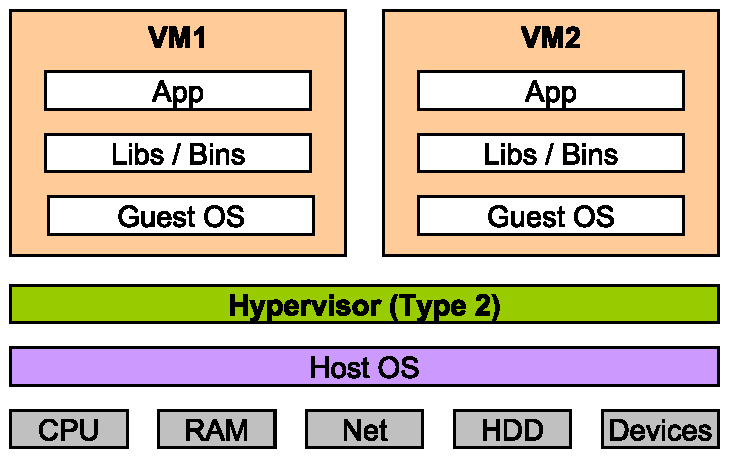
\includegraphics[scale=0.5]{figures/vm-hypervisor.pdf}
  \end{figure}
\end{frame}

\begin{frame}{Docker vs VM}
  \begin{itemize}
    \item \sout{Hypervisor}
    \item \sout{Guest OS}
    \item {\btHL System calls to Linux Kernel}
  \end{itemize}
  \begin{figure}
    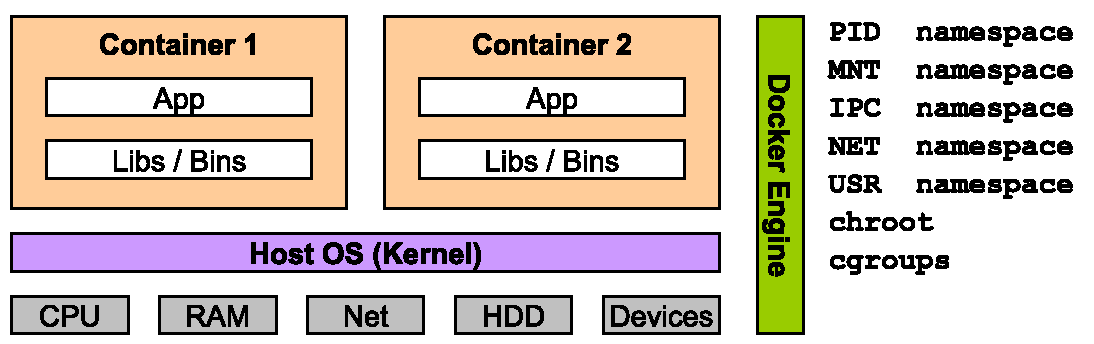
\includegraphics[scale=0.5]{figures/vm-docker.pdf}
  \end{figure}
\end{frame}

\section{Docker Commands}

\begin{frame}[fragile]{Docker hello-world}  
  \begin{itemize}
    \item Docker {\it "run"} creates new container each time
  \end{itemize}
  \begin{lstlisting}[basicstyle=\ttfamily\small\color{myblue}]
    @docker run hello-world@

    Unable to find image 'hello-world:latest' locally
    latest: Pulling from library/hello-world
    d1725b59e92d: Pull complete
    Digest: sha256:0add3ace90e
    Status: Downloaded newer image 

    Hello from Docker!
  \end{lstlisting}  
  \begin{itemize}
    \item Run detached process --- background mode
  \end{itemize}
  \begin{lstlisting}[basicstyle=\ttfamily\small\color{myblue}]
    docker run @--detach@ --name web nginx:latest
  \end{lstlisting}
\end{frame}

\begin{frame}[fragile]{Docker interactive}
\begin{itemize}
    \item Docker "run -it" in interactive mode
    \item Attach to STDIN/STDOUT
    \item Attach terminal to STDIN/STDOUT
  \end{itemize}  
  \begin{lstlisting}[basicstyle=\ttfamily\color{myblue}]
    docker run @--interactive --tty@ \
               busybox:latest /bin/sh
  \end{lstlisting}
\end{frame}

\begin{frame}[fragile]{Docker Commands And Lifecycle}
  \begin{itemize}
    \item create / start / stop / kill / restart / rm / exec / logs
  \end{itemize}
  \begin{figure}
    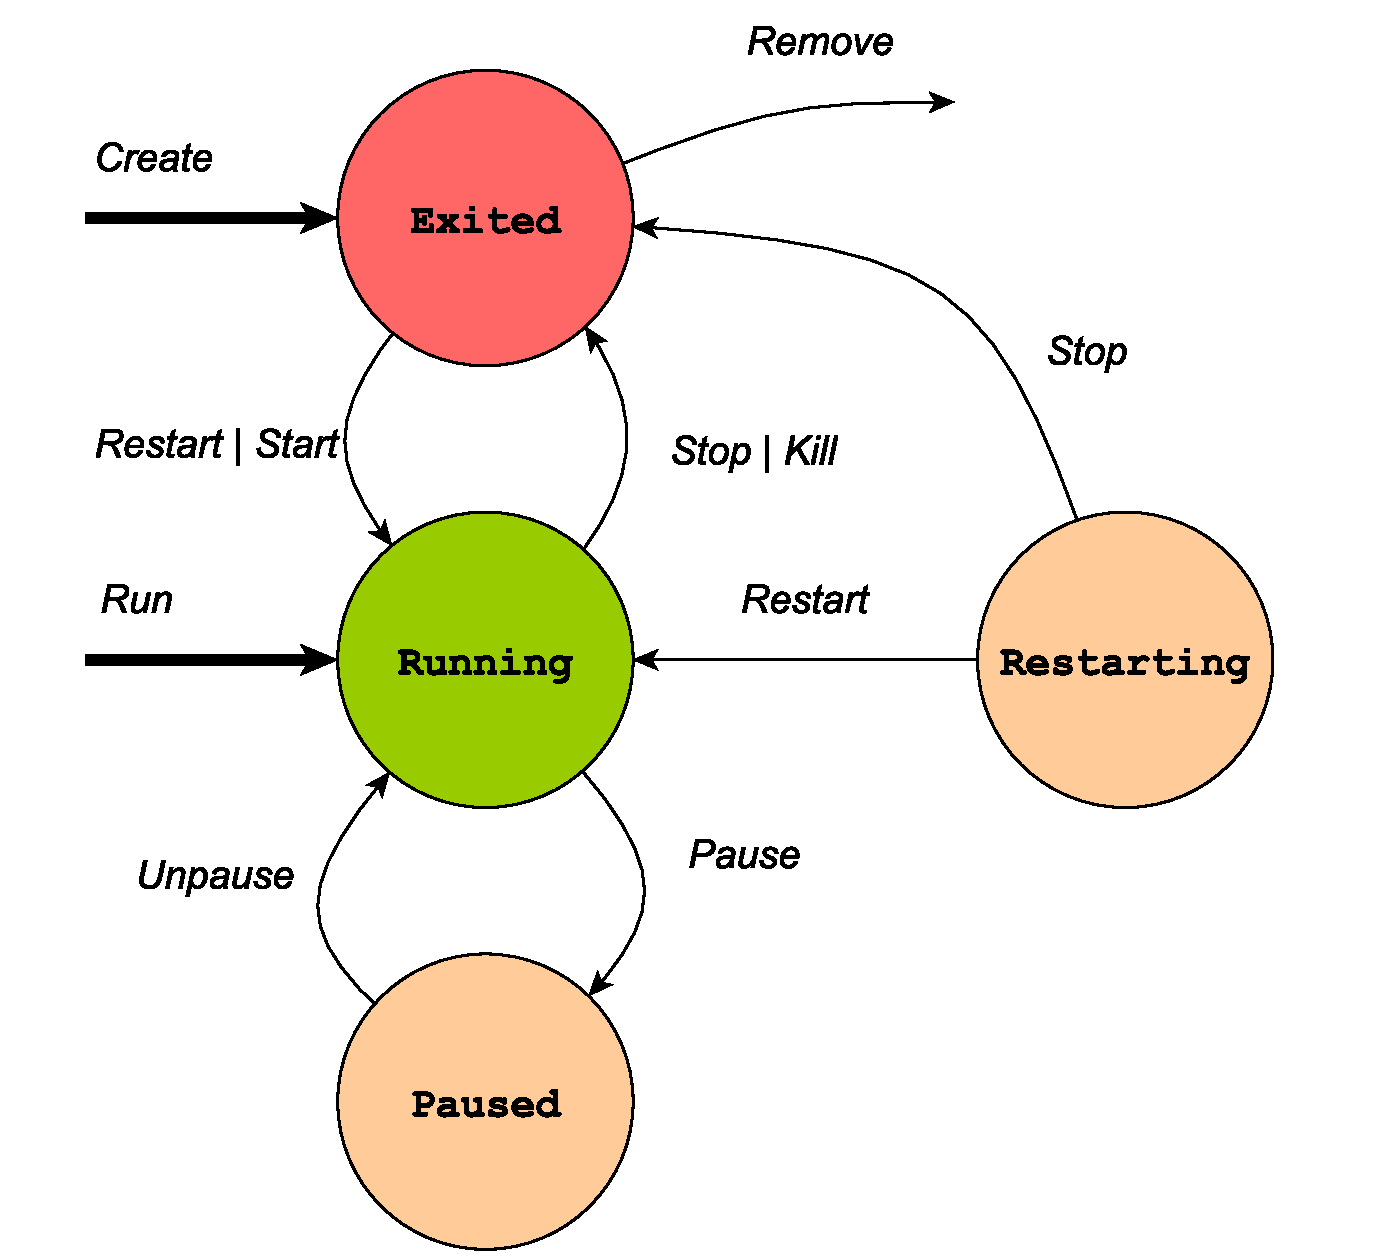
\includegraphics[scale=0.3]{figures/container-states.pdf}
  \end{figure}
\end{frame}

\begin{frame}[fragile]{Docker PS (-a)}
  \begin{itemize}
    \item The container ID
    \item The image used
    \item The command executed in the container
    \item The time since the container was created
    \item The duration that the container has been running
    \item The network ports exposed by the container
    \item The name of the container
  \end{itemize}
  \begin{lstlisting}[basicstyle=\ttfamily\tiny\color{myblue}]
    CONTAINER ID  IMAGE                   COMMAND             CREATED
    379f56c48527  grafana/grafana:5.0.3   "/run.sh"           3 weeks ago  
    a58b3427eda6  prom/prometheus:v2.2.1  "/bin/prometheus"   3 weeks ago  
    0c64881769f9  stressy:latest         " java "   3 weeks ago  
  \end{lstlisting}
  \begin{lstlisting}[basicstyle=\ttfamily\tiny\color{myblue}]
    STATUS      PORTS      NAMES
    Up 3 weeks  0.0.0.0:3002->3000/tcp  stressy-grafana
    Up 3 weeks  0.0.0.0:9092->9090/tcp  stressy-prometheus
    Exited (137)                        stressy
  \end{lstlisting}
\end{frame}

\begin{frame}[fragile]{Docker Commands Examples}  
  \begin{itemize}
    \item Read Only Image + Volumes
  \end{itemize}
  \begin{lstlisting}[basicstyle=\ttfamily\small\color{myblue}, frame=single]
    docker run -d --name test \
           @-v /run/lock/test/@ @--read-only@ \
          busybox:latest
  \end{lstlisting}
  \begin{itemize}
    \item Environment variables
  \end{itemize}
  \begin{lstlisting}[basicstyle=\ttfamily\small\color{myblue}, , frame=single]
    docker run @--env TEST_ENV_VAR="test"@ \
               busybox:latest env
  \end{lstlisting}  
\end{frame}

\begin{frame}[fragile]{Docker Commands Examples}  
  \begin{itemize}
    \item Linking containers (Deprecated!!!)
  \end{itemize}
  \begin{lstlisting}[basicstyle=\ttfamily\small\color{myblue}, , frame=single]
    docker run -d --name db -v /var/db/data db:latest
    
    docker create --name=reader1 @--link db@ \
                    db-reader:latest

    docker create --name=reader2 @--link db@ \
                    db-reader:latest
  \end{lstlisting}  
  \begin{itemize}
    \item Expose port
  \end{itemize}
  \begin{lstlisting}[basicstyle=\ttfamily\small\color{myblue}, frame=single]
    docker run --detach --name web @-p 80@ nginx:latest
  \end{lstlisting}       
\end{frame}

\begin{frame}[fragile]{Docker Commands Examples} 
  \begin{itemize}
    \item Override entrypoint
  \end{itemize}
  \begin{lstlisting}[basicstyle=\ttfamily\small\color{myblue}, frame=single]
    docker run -ti @--entrypoint=sh@ nginx:latest
  \end{lstlisting}    
  \begin{exampleblock}{Troubleshooting}
  Usefull for troubleshooting to override entrypoint and "look" into container if it fails to start, for example
  \end{exampleblock}
\end{frame}

\begin{frame}[fragile]{Docker Containers Automatic Restart}
  \begin{itemize}
    \item Never restart (default) --- no
    \item Restart when a failure is detected --- on-failure
    \item Restart when a failure is detected unless it explicitely stopped --- unless-stopped
    \item Always restart the container regardless of the condition --- always
  \end{itemize}  
  \begin{lstlisting}[basicstyle=\ttfamily\small\color{myblue}]
    docker run @--restart=always@ \
               busybox:latest env
  \end{lstlisting}  
\end{frame}

\begin{frame}{Docker Container Commands Recap}
  \begin{itemize}
    \item create --- create a container from an image
    \item start  --- start an existing container
    \item run    --- create a new container and start it
    \item ps     --- list running containers
    \item logs   --- print container logs
    \item stop   --- gracefully stop running container
    \item kill   --- stop main process in container container abruptly
    \item rm     --- remove stopped container
  \end{itemize}    
\end{frame}

\section{Docker Images}

\begin{frame}[fragile]{Dockerfile}
  \begin{exampleblock}{Dockerfile}
  Set of instructions which say how to build Docker image consisting of base image, filesystem layers, environment variable and instructions to run application
  \end{exampleblock}
\end{frame}

\begin{frame}[fragile]{Dockerfile}
  \begin{lstlisting}[basicstyle=\ttfamily\tiny\color{myblue}, , frame=single]
    # base image
    FROM docker.in.devexperts.com/ria/ria-openjdk:8u151-jdk-alpine3.7
    
    # add metadata for searching and identification
    LABEL "maintainer"="dtimofeev@devexperts.com"
    LABEL "appserver"="Tomcat"
    
    # set environment variables
    ENV CATALINA_HOME /usr/local/tomcat
    ENV PATH $CATALINA_HOME/bin:$PATH
    RUN mkdir -p "$CATALINA_HOME"
    WORKDIR $CATALINA_HOME

    ENV TOMCAT_NATIVE_LIBDIR $CATALINA_HOME/native-jni-lib
    ENV LD_LIBRARY_PATH ${LD_LIBRARY_PATH:+$LD_LIBRARY_PATH:}$TOMCAT_NATIVE_LIBDIR

    ENV TOMCAT_MAJOR 8
    ENV TOMCAT_VERSION 8.0.41

    ENV TOMCAT_TGZ_URL http://archive.apache.org/dist/tomcat/tomcat-$TOMCAT_MAJOR/v$TOMCAT_VERSION/bin/apache-tomcat-$TOMCAT_VERSION.tar.gz

    RUN apk --update add tar

    RUN wget -O tomcat.tar.gz "$TOMCAT_TGZ_URL" \
        && tar -xvf tomcat.tar.gz --strip-components=1 \
        && rm tomcat.tar.gz*

  \end{lstlisting}  
\end{frame}

\begin{frame}{Several Dockerfile commands}
  \begin{itemize}
    \item FROM  --- specifies base image
    \item LABEL --- provides metadata
    \item ENV   --- sets environmental variables
    \item RUN   --- runs command and creates image layer
    \item COPY  --- copies files and directories to the image
    \item ADD   --- copies files and directories to the image. Unpacks .tar files
    \item CMD   --- sets a command/arguments for an executing container. Parameters can be overridden. There can be only one CMD
    \item ARG   --- defined a variable to pass to Docker at build-time
    \item EXPOSE --- exposes a port
    \item VOLUME --- creates a directory mount point to access and store persistent data
    \item ENTRYPOINT --- configures command which runs each time a container is started
  \end{itemize}    
\end{frame}

\begin{frame}[fragile]{Docker Image Build}
  \begin{lstlisting}[basicstyle=\ttfamily\small\color{myblue}, , frame=single]
    Removing intermediate container 4e76a27d0987
    Step 3/13 : ENV CATALINA_HOME /usr/local/tomcat
     ---> @Running in 9e95902b7445@
     ---> @6ad788b83172@
    @Removing intermediate container 9e95902b7445@
    Step 4/13 : ENV PATH $CATALINA_HOME/bin:$PATH
     ---> Running in b4dbb019a07f
     ---> 2245940b88fe
    Removing intermediate container b4dbb019a07f
    Step 5/13 : RUN mkdir -p "$CATALINA_HOME"
     ---> Running in c33fddbaa99e
     ---> d580a8d4986c
    Removing intermediate container c33fddbaa99e
    Step 6/13 : WORKDIR $CATALINA_HOME
     ---> 418034d9a7d6
    Removing intermediate container 35f2929b5b51
  \end{lstlisting}  
\end{frame}

\begin{frame}[fragile]{Troubleshooting build}
In case of error during build process
\begin{lstlisting}[basicstyle=\ttfamily\small\color{myblue}, , frame=single]
    Removing intermediate container 4e76a27d0987
    Step 3/13 : ENV CATALINA_HOME /usr/local/tomcat
     ---> Running in 9e95902b7445
     ---> @6ad788b83172@
    Removing intermediate container 9e95902b7445
    Step 4/13 : ENV PATH $CATALINA_HOME/bin:$PATH
     ---> Running in b4dbb019a07f
          @ERROR!!!@
  \end{lstlisting}  
  \begin{exampleblock}{Troubleshoot}
  you can launch command in interactive mode in the last container before the error step
  \begin{lstlisting}[basicstyle=\ttfamily\tiny\color{myblue}, , frame=single]
    docker run --rm -ti @6ad788b83172@ /sh
  \end{lstlisting} 
  \end{exampleblock}
   
\end{frame}

\begin{frame}[fragile]{Keeping images small}
  \begin{itemize}
    \item Multi-goal commands --- creates only one additional layer    
  \end{itemize}  
  \begin{lstlisting}[basicstyle=\ttfamily\small\color{myblue}, , frame=single]
    RUN wget -O tomcat.tar.gz "$TOMCAT_TGZ_URL" 
        && tar -xvf tomcat.tar.gz --strip-components=1 
        && rm tomcat.tar.gz*
  \end{lstlisting}
\end{frame}

\begin{frame}[fragile]{Keeping images small}  
  \begin{itemize}
    \item Multi-stage builds
  \end{itemize}  
  \begin{lstlisting}[basicstyle=\ttfamily\tiny\color{myblue}, , frame=single]
    FROM golang:1.7.3 @as builder@
    WORKDIR /go/src/github.com/alexellis/href-counter/
    RUN go get -d -v golang.org/x/net/html  
    COPY app.go .
    RUN CGO_ENABLED=0 GOOS=linux go build -a -installsuffix cgo -o app .

    # use empty image
    FROM alpine:latest  
    RUN apk --no-cache add ca-certificates
    WORKDIR /root/
    # copy from builder container
    @COPY --from=builder /go/src/github.com/alexellis/href-counter/app .@
    CMD ["./app"]
  \end{lstlisting}  
\end{frame}

\begin{frame}[fragile]{Docker Image Layers }  
  \begin{lstlisting}[basicstyle=\ttfamily\tiny\color{myblue}, , frame=single]
    docker @history@ docker.in.devexperts.com/ria/tomcat
    IMAGE         CREATED        CREATED BY                       SIZE
    35cc64ce1494  5 months ago   wget -O tomcat.tar.gz $TOMCAT_   13.3 MB
    <missing>     5 months ago   apk --update add tar             1.76 MB
    <missing>     5 months ago   ENV TOMCAT_TGZ_URL=http...       0 B
    <missing>     5 months ago   ENV TOMCAT_VERSION=8.0.41        0 B
    <missing>     5 months ago   ENV TOMCAT_MAJOR=8               0 B
    <missing>     5 months ago   ENV LD_LIBRARY_PATH=/us...       0 B
    <missing>     5 months ago   ENV TOMCAT_NATIVE_LIBDI...       0 B
    <missing>     5 months ago   WORKDIR /usr/local/tomcat        0 B
    <missing>     5 months ago   mkdir -p $CATALINA_HOME          0 B
    <missing>     5 months ago   ENV PATH=/usr/local/tom...       0 B
    <missing>     5 months ago   ENV CATALINA_HOME=/usr/...       0 B
    <missing>     5 months ago   MAINTAINER Denis Timofe...       0 B
    <missing>     5 months ago   ENTRYPOINT [/usr/bin/d...        0 B
    <missing>     5 months ago   apk add --no-cache dumb-init     137 kB
    <missing>     5 months ago   MAINTAINER Denis Timofe...       0 B
    <missing>     6 months ago   set -x  && apk add --no-cache    97.4 MB
    ...
  \end{lstlisting}  
\end{frame}

\begin{frame}{Docker Image Commands Recap}
  \begin{itemize}
    \item build   --- build an image
    \item login   --- login to a remote repository
    \item push    --- push an image to a remote repository
    \item images  --- list all downloaded/built images
    \item history --- intermediate image info
    \item inspect --- info about the image
    \item rmi     --- delete image
  \end{itemize}    
\end{frame}

\section{Docker Mount Points}

\subsection{Docker Bind Mount Points}

\begin{frame}[fragile]{Docker Bind Mount Point }
  \begin{lstlisting}[basicstyle=\ttfamily\small\color{myblue}, , frame=single]
  docker run -d @-v ./host-folder:/data:ro@ alpine...
  \end{lstlisting}  
  \begin{figure}
    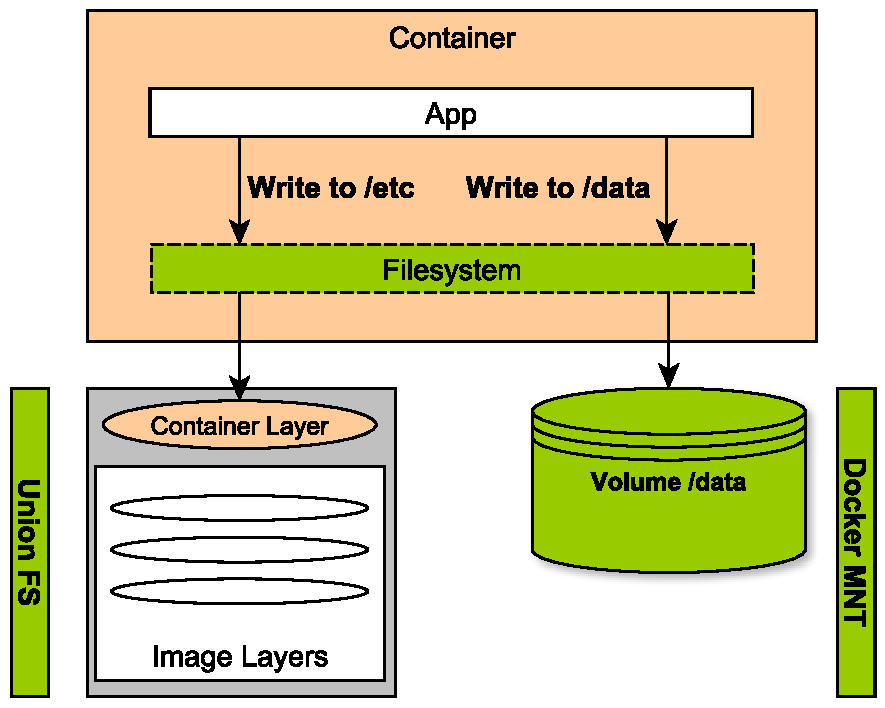
\includegraphics[scale=0.5]{figures/volumes.pdf}
  \end{figure}  
\end{frame}

\begin{frame}[fragile]{Union FS }    
  \begin{alertblock}{Union FileSystem}
  Docker Storage Drivers: overlay2, aufs, devicemapper, btrfs, zfs, vfs
  \end{alertblock}
  \begin{figure}
    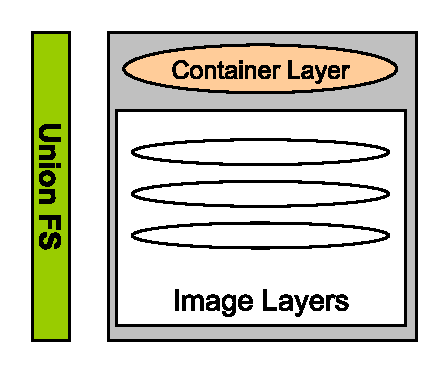
\includegraphics[scale=0.5]{figures/unionfs.pdf}
  \end{figure}
  \begin{alertblock}{Memmory-mapped files}
  If your application uses memmory-mapped files it's better to place them in bind-mount volume
  \end{alertblock}
\end{frame}

\begin{frame}[fragile]{Docker Bind Mount File }
 \begin{lstlisting}[basicstyle=\ttfamily\color{myblue}, , frame=single]
    docker run -d  
          @-v ./folder/test.txt:/folder/text.txt:ro@
          alpine...
  \end{lstlisting}
  \begin{alertblock}{Existing file}
  File MUST exist in image which is used for container. Otherwise new directory will be created and named with filename
  \end{alertblock}
\end{frame}

\subsection{Docker Managed Volume}

\begin{frame}[fragile]{Docker Managed Volume }
  \begin{lstlisting}[basicstyle=\ttfamily\small\color{myblue}, , frame=single]
  docker run -d @--volume /var/lib/data@ --name data-shared alpine...

  docker run -d @--volumes-from data-shared@ busybox...
  \end{lstlisting}
  \begin{figure}
    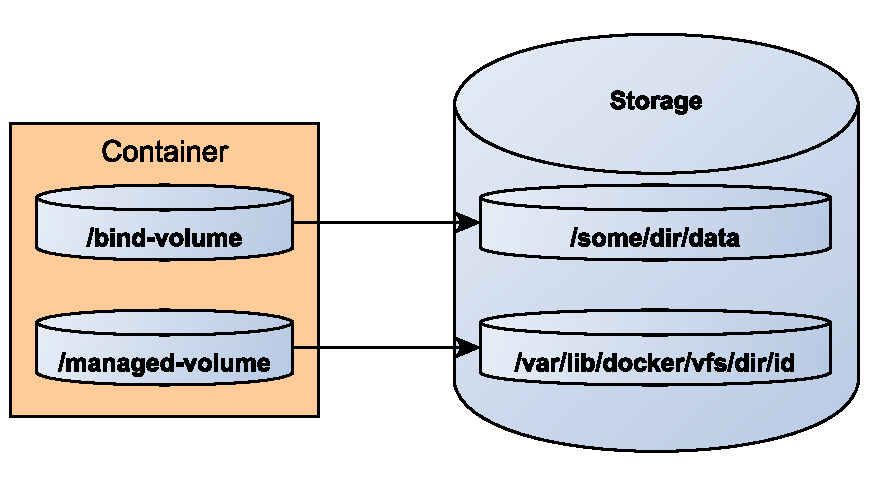
\includegraphics[scale=0.5]{figures/managed-volume.pdf}
  \end{figure}
\end{frame}

\section{Docker Networking}

\subsection{Closed Container}

\begin{frame}[fragile]{Closed Container}
  \begin{lstlisting}[basicstyle=\ttfamily\tiny\color{myblue}, , frame=single]
  docker run --rm @--net none@ busybox ip addr
  \end{lstlisting}
  \begin{itemize}
    \item Doesn't allow any network traffic
  \end{itemize}  
  \begin{figure}
    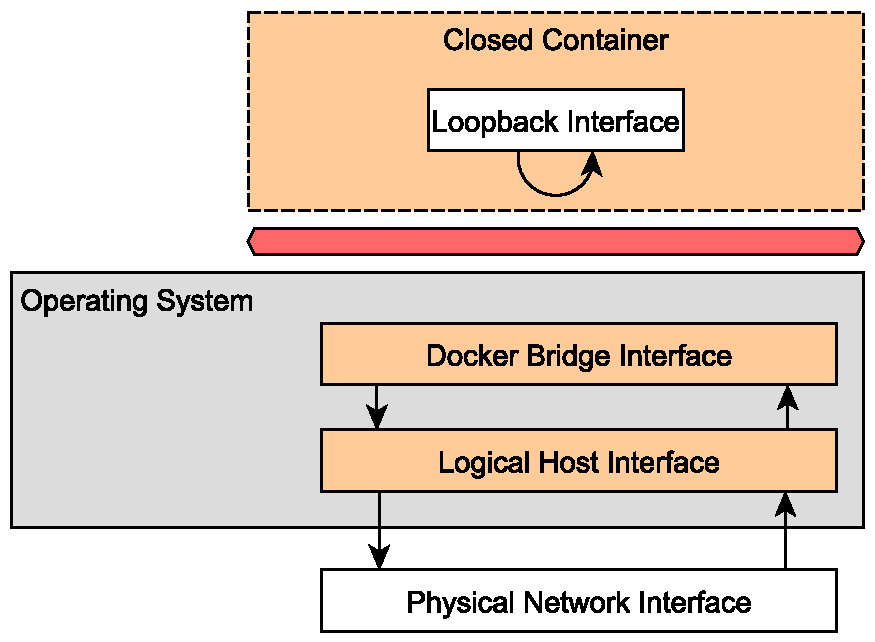
\includegraphics[scale=0.5]{figures/net-closed-container.pdf}
  \end{figure}
\end{frame}

\subsection{Bridged Container}

\begin{frame}[fragile]{Bridged Container}
  \begin{lstlisting}[basicstyle=\ttfamily\tiny\color{myblue}, , frame=single]
    docker run --rm @--net bridge@ busybox ip addr
    docker run --rm @--net bridge@ -p 8080:80 busybox ip addr
    docker run --rm @--net bridge@ --hostname=busy busybox ip addr
  \end{lstlisting}
  \begin{itemize}
    \item Allows access to network / containers can be found using their ip addresses
  \end{itemize}  
  \begin{figure}
    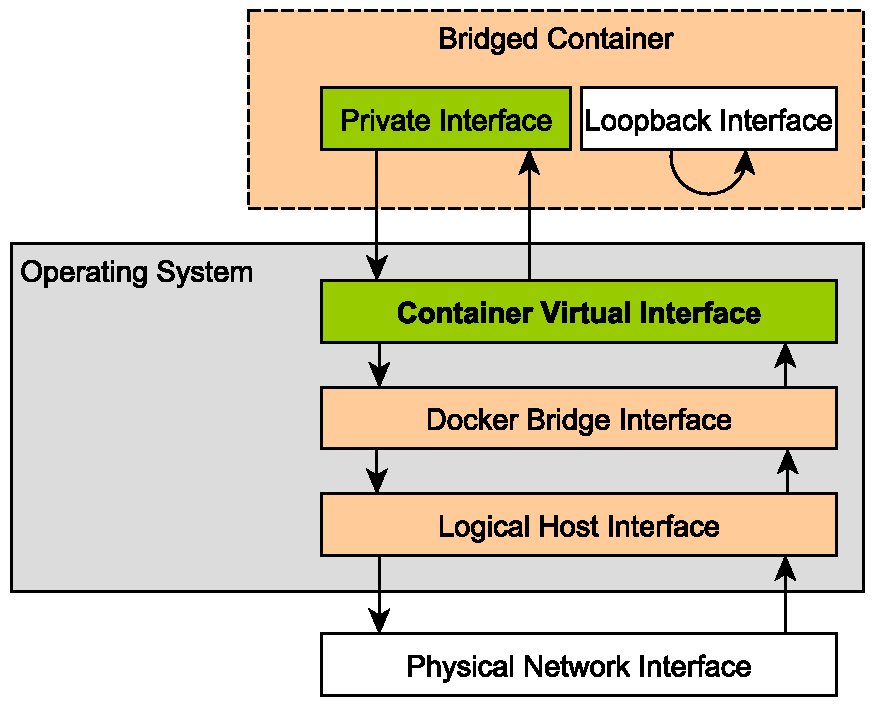
\includegraphics[scale=0.4]{figures/net-bridged-container.pdf}
  \end{figure}
\end{frame}

\subsection{Joined Container}

\begin{frame}[fragile]{Joined Container}
  \begin{lstlisting}[basicstyle=\ttfamily\tiny\color{myblue},frame=single]
    docker run --rm @--net none --name foo@ busybox ip addr
    docker run --rm @--net container:foo@ --name bar busybox ip addr
  \end{lstlisting}
  \begin{itemize}
    \item Allows access to container's network stack
  \end{itemize} 
  \begin{figure}
    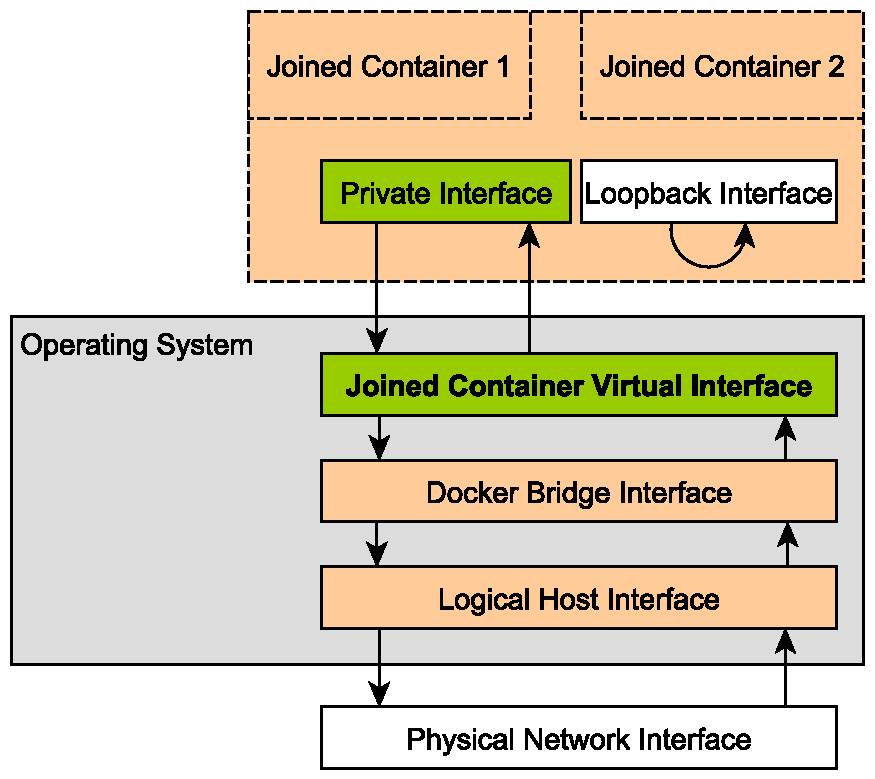
\includegraphics[scale=0.4]{figures/net-joined-containers.pdf}
  \end{figure}
\end{frame}

\subsection{Open Container}

\begin{frame}[fragile]{Open Container}
  \begin{lstlisting}[basicstyle=\ttfamily\tiny\color{myblue},frame=single]
    docker run --rm @--net host@ busybox ip addr
  \end{lstlisting}
  \begin{figure}
    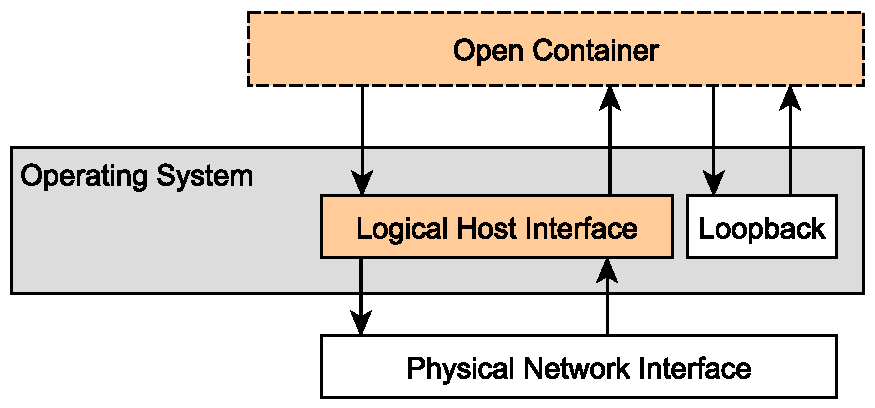
\includegraphics[scale=0.5]{figures/net-open-container.pdf}
  \end{figure}
\end{frame}

\subsection{Containers Linking}

\begin{frame}[fragile]{Containers Linking}
  \begin{itemize}
    \item Sets env variables describing target container's endpoint (env sharing)
    \item Adds link allias to the DNS override list
    \item If inter-container communication (ICC) is disabled adds specific firewall rules to allow communication between containers ("expose" flag)    
  \end{itemize}  
  \begin{lstlisting}[basicstyle=\ttfamily\tiny\color{myblue},frame=single]
    docker run -d --name db -v /var/db/data db:latest
    
    docker create --name=reader1 @--link db@ db-reader:latest
    docker create --name=reader2 @--link db@ db-reader:latest
  \end{lstlisting}  
  \begin{alertblock}{Links are deprecated}
  Use user-defined bridges instead
  \end{alertblock}
\end{frame}

\subsection{User-defined bridges}

\begin{frame}[fragile]{User-defined bridges}  
  \begin{lstlisting}[basicstyle=\ttfamily\small\color{myblue}]
    docker @network create@ my-net
    
    docker create --name my-nginx @--network my-net@ \
                  --publish 8080:80 nginx:latest
  \end{lstlisting} 
  \begin{itemize}
    \item Better isolation and interoperability between containerized applications (less open ports)
    \item Automatic DNS resolution between containers
    \item Containers can be attached and detached from user-defined networks on the fly (stop/recreate on defaul bridge)
    \item Linked containers on the user-defined bridge network doesn't share environment variables
  \end{itemize}  
\end{frame}

\begin{frame}[fragile]{User-defined bridges}  
  \begin{alertblock}{User-defined network subnet}
    Always set subnet for user-defined network. By default docker chooses subnet itself and can choose one conflicting with your infrastructure. Hello, IP tables!
  \end{alertblock} 
  \begin{lstlisting}[basicstyle=\ttfamily\small\color{myblue}]
    docker network create stress-test
           --driver=bridge \
           --ipam-driver=default \
           @--subnet=172.32.0.0/12@
  \end{lstlisting}    
\end{frame}

\section{Resource Allowance}

\begin{frame}{Resource Allowance}
  \begin{itemize}
    \item Memmory --- the amount of memmory container can use (memory)
    \item CPU     --- CPU shares container can use (cpu-shares)
    \item CPU set --- assign CPU for container - cache friendly (cpuset-cpus)
    \item Devices --- allow container to use host's devices (device)
    \item Shared Memmory --- allow IPC (ipc)  
    \item User space --- user option
  \end{itemize}
\end{frame}

\section{Feature Authorizations}

\begin{frame}{Feature Authorizations}
  \begin{block}{OS capabilities}
  When a process makes system calls, the capabilities of that process are checked for the required capability. The required call will succeed if the process has the requireds capability and fail otherwise
  \end{block}
  \begin{itemize}
    \item SYS\_NICE --- Modify priority of processes
    \item SYS\_RESOURCE --- Override resource limits
    \item SYS\_TIME --- Modify the system clock
    \item SYS\_TTY\_CONFIG --- Configure TTY devices 
    \item ...
  \end{itemize}  
  \begin{exampleblock}{Defaults}
  By default Docker drops a set of capabilities to enforce isolation from administrative functions (cap-drop/cap-add)
  \end{exampleblock}
\end{frame}

\section{Full privileges mode}

\begin{frame}{Full privileges mode}
  \begin{itemize}
    \item Use --privileged flag
    \item Still partially isolated --- network namespace still works
    \item Use --net host to drop network isolation
  \end{itemize}
  \begin{exampleblock}{God mode}
  Process looks like "uncontainerized" one but you still get all the tooling from Docker related to container management
  \end{exampleblock}
\end{frame}

\end{document}


